\documentclass[11pt,mathserif]{beamer}

% !!! pour compiler (en francais)
% (1) latex soutenance
% (2) dvips -Ppdf -G0 soutenance
% (3) ps2pdf soutenance.ps

% !!! pour compiler (en anglais)
% (1) latex siopt
% (2) dvips siopt.dvi -u +psfonts.cmz -o
% (3) ps2pdf siopt.ps


%% ====== packages ==
%\usepackage{../../../inputs/style-article/police-speciale-bouquin}
%\usepackage{../../../inputs/style-article/enumeration-bouquin}
%\usepackage{commande-hk-bouquin}
%\usepackage{../../../inputs/style-article/mathematique-bouquin}
%\usepackage{ifthen} % pour commande-hk-bouquin
\usepackage{amsmath,amssymb,amsfonts}
%\usepackage{style-rticle/mise-en-page-bouquin}  % un petit souci de caption
\usepackage{graphicx}
\newcommand{\tiret}{\rule[0.6ex]{1.3ex}{0.22ex}}

% !! pour le francais
\usepackage[latin1]{inputenc}
\usepackage{listings}
%\usepackage[ec]{aeguill}
% ou mieux \usepackage[cyr]{aeguill} si disponible
% aeguill charge ae automatiquement
% et ae charge [T1]{fontenc} automatiquement
\usepackage[french]{babel}
\usepackage{algpseudocode}
\usepackage{relsize}
\newcommand{\fleche}{\alert{$\pmb{\longrightarrow}$}~~}
\newcommand{\calM}{{\mathcal{M}}}
\newcommand{\calU}{{\mathcal{U}}}
\newcommand{\Cau}{\mathcal{C}_{n+1}}
\newcommand{\R}{\mathbb{R}}
\newcommand{\Sym}[1]{\mathcal{S}_{#1}(\R)}
\newcommand{\tran}{^{\top}}
\newcommand{\pssg}{\langle \langle}
\newcommand{\pssd}{\rangle \rangle}
\newcommand{\aronde}{\mathcal{A}}
\newcommand{\Tr}{\mathtt{Tr}}
\newcommand{\Matr}[1]{\mathcal{M}_{#1}(\R)}
\newcommand{\calV}{{\mathcal{V}}}
\newcommand{\calS}{{\mathcal{S}}}
\newcommand{\corra}{{\mathrm{corr}_a}}
\newcommand{\rmD}{{\mathrm{D}}}
\newcommand{\rmN}{{\mathrm{N}}}
\newcommand{\rmP}{{\mathrm{P}}}
\newcommand{\rmT}{{\mathrm{T}}}
\def\Sy{{\cal S}_n}
\newcommand{\accol}[1]{{\left\{ \begin{array}{ll} #1 \end{array} \right.}}
\newcommand{\prods}[2]{\langle #1,#2 \rangle}
\newcommand{\Aa}{\mathcal{A}}
\newcommand{\norm}[1]{\|#1\|}
\newcommand{\python}{\textcolor{dkgreen}{\bf Python}{} }

%% ====== my bearmer ==
\mode<presentation> {
\usetheme{default}    % sobre
%\usetheme{Pittsburgh}  % default avec un titre a droite
%\usetheme{Singapore}   % avec une table-of-contens-sildebar

% options
\useinnertheme[shadow]{rounded}  % les numeros
}
\definecolor{dkgreen}{rgb}{0,0.6,0}
\definecolor{gray}{rgb}{0.5,0.5,0.5}
\definecolor{mauve}{rgb}{0.58,0,0.82}


\usefonttheme{structurebold}

\lstset{ %
  language=python,                % the language of the code
  framerule=0pt,
  basicstyle=\relsize{-2}\ttfamily,  % the size of the fonts that are used for the code
  %backgroundcolor=\color{black!10},  % choose the background color. You must add \usepackage{color}
  showspaces=false,               % show spaces adding particular underscores
  showstringspaces=false,         % underline spaces within strings
  showtabs=false,                 % show tabs within strings adding particular underscores
  %frame=single,                   % adds a frame around the code
  rulecolor=\color{black},        % if not set, the frame-color may be changed on line-breaks within not-black text (e.g. commens (green here))
  breakatwhitespace=false,        % sets if automatic breaks should only happen at whitespace
  keywordstyle=\color{blue},      % keyword style
  commentstyle=\color{dkgreen},   % comment style
  stringstyle=\color{mauve}  
}

%%%%%%%%%%%%%%%%%%%%%%%%%
% Francisation du pseudo code
%%%%%%%%%%%%%%%%%%%%%%%%%
\algrenewcommand\algorithmicif{\textbf{si}}
\algrenewcommand\algorithmicend{\textbf{fin}}
\algrenewcommand\algorithmicelse{\textbf{sinon}}
\algrenewcommand\algorithmicwhile{\textbf{tant que}}
\algrenewcommand\algorithmicthen{\textbf{alors}}
\algrenewcommand\algorithmicfor{\textbf{pour}}
\algrenewcommand\algorithmicfor{\textbf{retouner}}
\algrenewcommand\algorithmicdo{\textbf{faire}}


\begin{document}

%****************************************************************
% Page de presentation 
%**************************************************************
\begin{frame}
\begin{center}
{\Large Initiation a la Programmation avec Python } 
\end{center}
%\begin{center}
%\includegraphics[width=0.3\linewidth]{Fig/gdb}
%\end{center}
\begin{center}
{\large Inria Bordeaux-Sud Ouest \\ F�te de la Science 2013}
\end{center}
\end{frame}

%****************************************************************
% Plan 
%**************************************************************

\begin{frame}
\frametitle{Plan}

\begin{enumerate}
\item Qu'est ce que la programmation 
\item Exemples 
\item Python
   \begin{itemize}
    \item donn�es python
    \item structures de contr�le. 
   \end{itemize}
\end{enumerate}

\end{frame}

%%%%%%%%%%%%%%%%%%%%%%%%%%%%%%%%%%%%%%%%%%%%%%%%%%%%%%%%%%%%%%%%%%
%
%%%%%%%%%%%%%%%%%%%%%%%%%%%%%%%%%%%%%%%%%%%%%%%%%%%%%%%%%%%%%%%%%%%

%****************************************************************
%  example 1
%****************************************************************
\begin{frame}
\frametitle{Exemple : somme des $n$ premiers entiers}
\begin{itemize}[<+->]
  \item l'algorithme peut ressembler a ca : 
   \begin{description}
      \item[1.] dans une case m�moire (variable) je mets 1
      \item[2.] au contenu de la case m�moire j'atoute 2
      \item[2.] au contenu de la case j'atoute 3 
      \item[...] .....
      \item[n.] au contenu de la case m�moire j'atoute $n$ 
      \item[n+1.] je retourne le contenu de la case m�moire
   \end{description}
\end{itemize}
\end{frame}

%****************************************************************
%  example 1
%****************************************************************
\begin{frame}[fragile]
\frametitle{Exemple : somme des $n$ premier entiers}
\begin{itemize}
  \item On peut formaliser l'{\bf algorithme} avec du {\em pseudo-code}
   \begin{algorithmic}
   \State{$s \gets 1$}
   \For{$i\gets 2,n$} 
     \State{$s \gets s + i$}
   \EndFor
   \State{afficher $s$}
   \end{algorithmic}
\item Ce qui donne en \python
\begin{lstlisting} 
    s = 1  
    for i in range(n):
        s = s + i
    print s
\end{lstlisting}
\end{itemize}
\end{frame}
%****************************************************************
% Remarques g�n�rales sur Python 
%****************************************************************
\begin{frame}[fragile]
\frametitle{Caract�ristiques du langage \python}
\begin{itemize}
  \item \python est un langage interpr�t� : on peut modifier
  dynamiquement (� la vol�e) le code du programme.
  \item la structure du programme se g�re gr�ce � des indentations : attention � aligner
  les blocs avec le m�me nombre d'espace
\begin{columns}
\column{0.4\linewidth}
{\bf Correct} 
\begin{lstlisting}
i = 1  
while i < 10 : 
    i = i * 2
    j = i - 2
\end{lstlisting}
\column{0.4\linewidth}
{\bf pas bien }
\begin{lstlisting}
  i = 1  
while i < 10 : 
    i = i * 2
  j = i - 2
\end{lstlisting}
\end{columns}
\end{itemize}
\end{frame}
\begin{frame}[fragile]
\frametitle{Le premier programme}
\begin{itemize}
 \item Quand on commence a apprendre un langage informatique, la ``tradition'' veut que le premier
 programme qu'on �crit soit un programme affichant ``bonjour, monde''\footnote{Hello, World dans la langue de Shakespeare}
\item dans la console de {\bf spyder}, on ecrira
\begin{lstlisting}
print "bonjour, Monde"
\end{lstlisting}
\item ca doit ressembler � quelque chose comme
\begin{center}
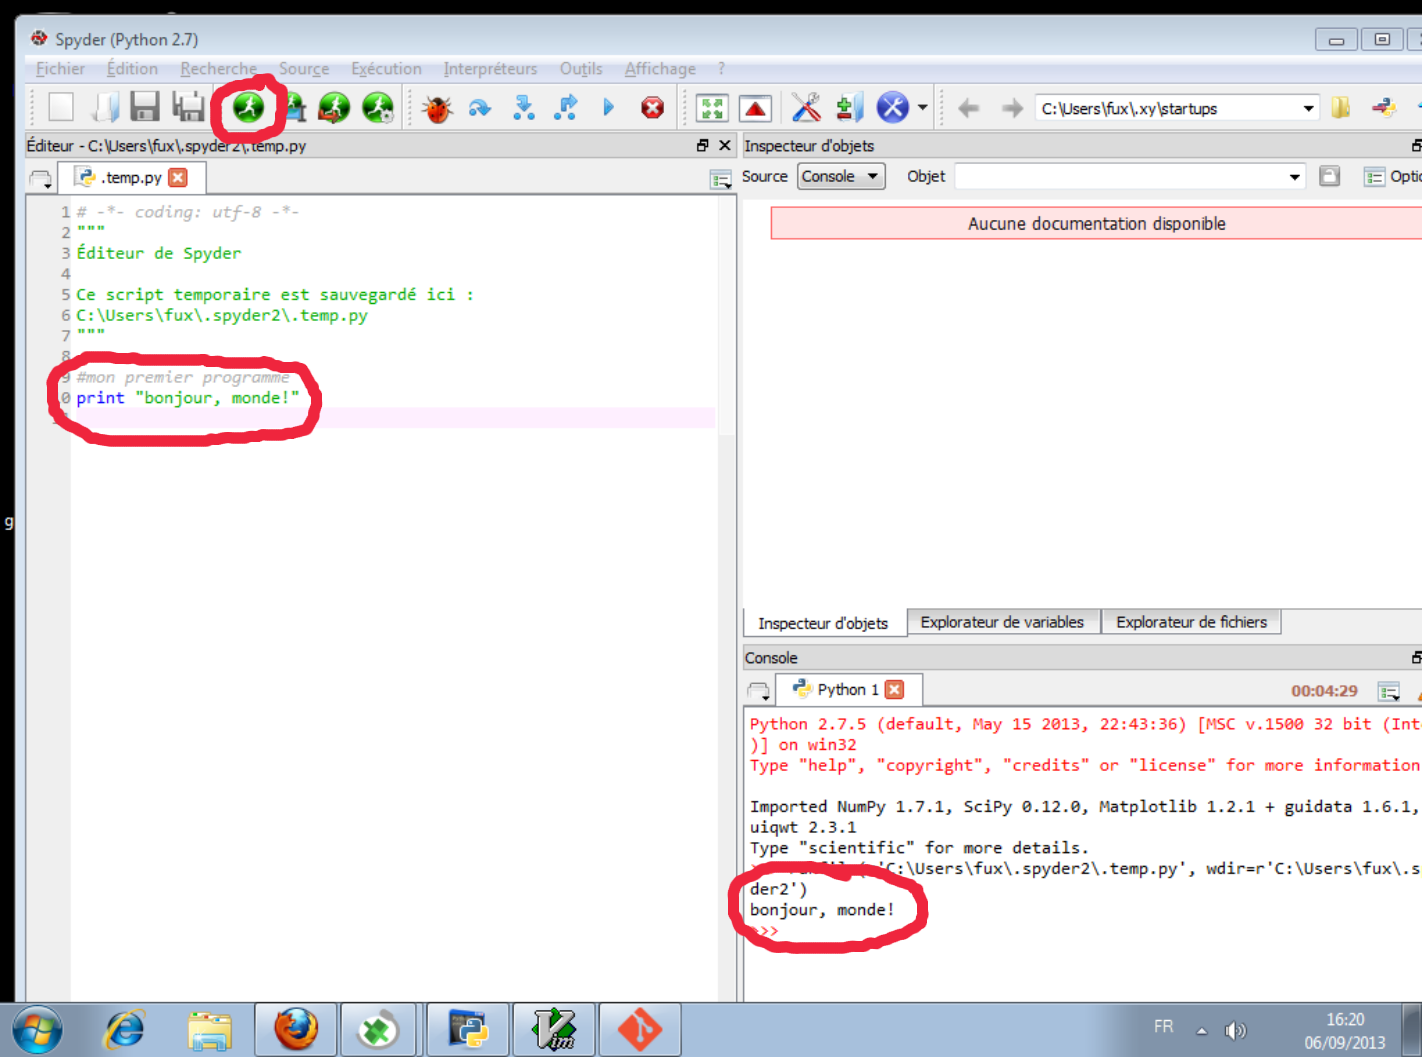
\includegraphics[width=0.7\linewidth]{capture_hello.png}
\end{center}
\end{itemize}
\end{frame}

\begin{frame}[fragile]
\frametitle{Structure de contr�le : branchement}
\begin{itemize}
 \item On peut avoir besoin dans un programme, selon un r�sultat
d'opter entre 2 ou plusieurs choix. 
\begin{algorithmic}
\If{ condition 1 } 
    \State{ action 1} 
\Else{ Condition 2 }    
    \State{ action 2}
\EndIf
\end{algorithmic}
\item en \python on fait comme cela
\begin{lstlisting}
if x < 1.50 :
   print('je suis petit')
elif  x < 1.80 :
   print('je suis moyen')
else:
   print('je suis grand')
\end{lstlisting}
\end{itemize}
\end{frame}

\begin{frame}[fragile]
\frametitle{Structure de contr�le : it�ration}
\begin{itemize}
 \item But : r�peter des t�ches sembabes
\item boucle {\bf tant que } : on boucle tant qu'une condition est vraie  
\begin{columns}
\column{0.4\linewidth}
\begin{algorithmic}
\State{$i \gets 1$} 
\While{ $i < 10$} 
    \State{ $i \gets 2 \times i$ } 
\EndWhile
\end{algorithmic}
\column{0.4\linewidth}
\begin{lstlisting}
i = 1  
while i < 10 : 
    i = i * 2
\end{lstlisting}
\end{columns}
\item boucle �numerative : on parcours un ensemble de valeurs 
\begin{columns}
\column{0.5\linewidth}
\begin{algorithmic}
\For{$i = 1, \cdots, 10 $} 
    \State{Afficher $i$}
\EndFor
\end{algorithmic}
\column{0.5\linewidth}
\begin{lstlisting}
for i in range(1,11): 
    print(i)  
\end{lstlisting}
\end{columns}

\end{itemize}
\end{frame}
\end{document}
